\newpage
\subsection{Paths, Walks, Cycles}
\begin{definition}[]{Paths, Walks, and Cycles in Graphs}
    \begin{itemize}
        \item \textbf{Walk:} A sequence of vertices and edges in a graph, where each edge connects consecutive vertices in the sequence. Vertices and edges may repeat.
        \item \textbf{Path:} A walk with no repeated vertices. In a directed graph, the edges must respect the direction.
        \item \textbf{Cycle:} A path that starts and ends at the same vertex. For a simple cycle, all vertices (except the start/end vertex) and edges are distinct.
        \item \textbf{Eulerian Walk:} A walk that traverses every edge of a graph exactly once.
        \item \textbf{Closed Eulerian Walk (Eulerian Cycle):} An Eulerian walk that starts and ends at the same vertex.
        \item \textbf{Hamiltonian Path:} A path that visits each vertex of a graph exactly once. Edges may or may not repeat.
        \item \textbf{Hamiltonian Cycle:} A Hamiltonian path that starts and ends at the same vertex.
    \end{itemize}
\end{definition}

\begin{properties}[]{Eulerian Graphs}
    \begin{itemize}
        \item \textbf{Undirected Graph:}
              \begin{itemize}
                  \item A graph has an Eulerian walk if it has exactly two vertices of odd degree (necessary condition).
                  \item A graph has a closed Eulerian walk if all vertices have even degree (necessary condition).
              \end{itemize}
        \item \textbf{Directed Graph:}
              \begin{itemize}
                  \item A graph has an Eulerian walk if at most one vertex has \textit{in-degree} one greater than its \textit{out-degree}, and at most one vertex has \textit{out-degree} one greater than its \textit{in-degree}. All other vertices must have equal in-degree and out-degree.
                  \item A graph has a closed Eulerian walk if every vertex has equal in-degree and out-degree.
              \end{itemize}
    \end{itemize}
\end{properties}

\begin{properties}[]{Hamiltonian Graphs}
    \begin{itemize}
        \item Unlike Eulerian walks, there is no simple necessary or sufficient condition for the existence of Hamiltonian paths or cycles.
        \item A graph with $n$ vertices is Hamiltonian if every vertex has a degree of at least $\lceil n / 2 \rceil$ (Dirac's Theorem, sufficient condition).
    \end{itemize}
\end{properties}

\begin{example}[]{Eulerian and Hamiltonian}
    \begin{center}
        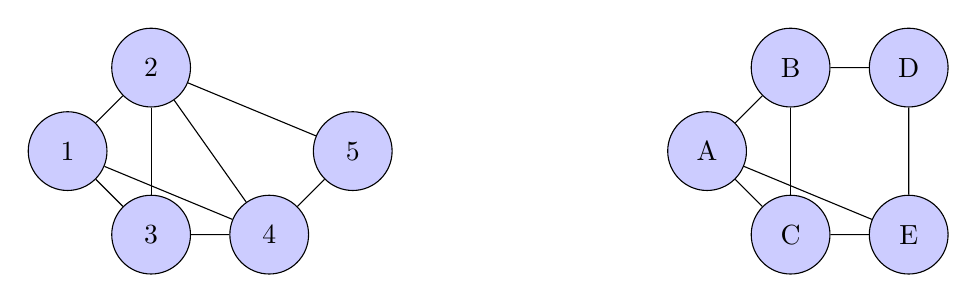
\begin{tikzpicture}[node distance=1.5cm, main/.style={circle, draw, fill=blue!20, minimum size=10mm, inner sep=0pt}] % Eulerian graph example
            \node[main] (1) {1};
            \node[main] (2) [above right of=1] {2};
            \node[main] (3) [below right of=1] {3};
            \node[main] (4) [right of=3] {4};
            \node[main] (5) [above right of=4] {5};
            \draw (1) -- (2) -- (5) -- (4) -- (3) -- (1) -- (4) -- (2);
            \draw (2) -- (3);

            % Hamiltonian graph example
            \node[main] (6) [right of=5, xshift=3cm] {A};
            \node[main] (7) [above right of=6] {B};
            \node[main] (8) [below right of=6] {C};
            \node[main] (9) [right of=7] {D};
            \node[main] (10) [right of=8] {E};
            \draw (6) -- (7) -- (9) -- (10) -- (8) -- (6);
            \draw (6) -- (10);
            \draw (7) -- (8);
        \end{tikzpicture}
    \end{center}
\end{example}

\begin{remarks}[]{Key Differences Between Eulerian and Hamiltonian Concepts}
    \begin{itemize}
        \item Eulerian paths are concerned with traversing every \textbf{edge} exactly once, while Hamiltonian paths are about visiting every \textbf{vertex} exactly once.
        \item Eulerian properties depend on the degree of vertices, whereas Hamiltonian properties depend on overall vertex connectivity.
    \end{itemize}
\end{remarks}
